\documentclass[a4paper,10pt,landscape]{article}
\usepackage[utf8]{inputenc}
\usepackage[ngerman]{babel}
\usepackage{amssymb,amsmath,amsthm,amsfonts}
\usepackage{multicol,multirow}
\usepackage{calc}
\usepackage{ifthen}
\usepackage{graphicx}
\usepackage[most]{tcolorbox}
\tcbuselibrary{breakable}
\graphicspath{ {images/} }
\usepackage[landscape]{geometry}
\usepackage{lipsum}
\usepackage[colorlinks=true,citecolor=blue,linkcolor=blue]{hyperref}
\usepackage{enumerate}

\ifthenelse{\lengthtest { \paperwidth = 11in}}
    { \geometry{top=.5in,left=.5in,right=.5in,bottom=.5in} }
	{\ifthenelse{ \lengthtest{ \paperwidth = 297mm}}
		{\geometry{top=1cm,left=1cm,right=1cm,bottom=1cm} }
		{\geometry{top=1cm,left=1cm,right=1cm,bottom=1cm} }
	}
\pagestyle{empty}

\makeatletter

\renewcommand{\section}{\@startsection{section}{1}{0mm}%
                                {-1ex plus -.5ex minus -.2ex}%
                                {0.5ex plus .2ex}%x
                                {\normalfont\large\bfseries}}
\renewcommand{\subsection}{\@startsection{subsection}{2}{0mm}%
                                {-1explus -.5ex minus -.2ex}%
                                {0.5ex plus .2ex}%
                                {\normalfont\normalsize\bfseries}}
\renewcommand{\subsubsection}{\@startsection{subsubsection}{3}{0mm}%
                                {-1ex plus -.5ex minus -.2ex}%
                                {1ex plus .2ex}%
                                {\normalfont\small\bfseries}}
\makeatother
\setcounter{secnumdepth}{0}
\setlength{\parindent}{0pt}
\setlength{\parskip}{0pt plus 0.5ex}

% breckman style
% Bruno Eckmann (nicht weiterverwenden)

\newcommand*{\Matlab}{\textsc{matlab}}
\newcommand*{\R}{\mathbb{R}}
\newcommand{\vek}[3]{\begin{pmatrix} #1 \\ #2 \\ #3 \end{pmatrix}}
\newcommand{\vekk}[2]{\begin{pmatrix} #1 \\ #2\end{pmatrix}}


\newtcbtheorem[]{Definition}{Definition}{
	enhanced,
	breakable,
	pad at break=1mm,
	break at=-\baselineskip/0pt,
	sharp corners,
	attach boxed title to top left={
		yshifttext=-1mm
	},
	colback=white,
	colframe=blue!25!white,
	fonttitle=\bfseries,
	coltitle=black,
	before skip=20pt,
	after skip=20pt,
	boxed title style={
		sharp corners=south,
		size=small,
		colback=blue!25!white,
		colframe=blue!25!white,
	} 
}{def}

\newtcbtheorem[]{Satz}{Satz}{
	enhanced,
	breakable,
	pad at break=1mm,
	break at=-\baselineskip/0pt,
	sharp corners,
	attach boxed title to top left={
		yshifttext=-1mm
	},
	colback=white,
	colframe=magenta!25,
	fonttitle=\bfseries,
	coltitle=black,
	before skip=20pt,
	after skip=20pt,
	boxed title style={
		sharp corners=south,
		size=small,
		colback=magenta!25,
		colframe=magenta!25,
	} 
}{stz}

\newtcbtheorem[no counter]{Diverses}{}{
	enhanced,
	breakable,
	pad at break=1mm,
	break at=-\baselineskip/0pt,
	sharp corners,
	attach boxed title to top left={
		yshifttext=-1mm
	},
	colback=white,
	colframe=magenta!25,
	fonttitle=\bfseries,
	coltitle=black,
	before skip=20pt,
	after skip=20pt,
	boxed title style={
		sharp corners=south,
		size=small,
		colback=magenta!25,
		colframe=magenta!25,
	} 
}{divs}

\newtcbtheorem[]{Rezept}{Rezept}{
	enhanced,
	breakable,
	pad at break=1mm,
	break at=-\baselineskip/0pt,
	sharp corners,
	attach boxed title to top left={
		yshifttext=-1mm
	},
	colback=white,
	colframe=yellow!55,
	fonttitle=\bfseries,
	coltitle=black,
	before skip=20pt,
	after skip=20pt,
	boxed title style={
		sharp corners=south,
		size=small,
		colback=yellow!55,
		colframe=yellow!55,
	} 
}{rzpt}

\newtcbtheorem[no counter]{Rechenregeln}{Nützliches}{
	enhanced,
	breakable,
	pad at break=1mm,
	break at=-\baselineskip/0pt,
	sharp corners,
	attach boxed title to top left={
		yshifttext=-1mm
	},
	colback=white,
	colframe=magenta!25,
	fonttitle=\bfseries,
	coltitle=black,
	before skip=20pt,
	after skip=20pt,
	boxed title style={
		sharp corners=south,
		size=small,
		colback=magenta!25,
		colframe=magenta!25,
	} 
}{stz}

\newtcbtheorem[]{Beispiel}{Beispiel}{
	enhanced,
	breakable,
	pad at break=1mm,
	break at=-\baselineskip/0pt,
	sharp corners,
	attach boxed title to top left={
		yshifttext=-1mm
	},
	colback=white,
	colframe=green!25,
	fonttitle=\bfseries,
	coltitle=black,
	before skip=20pt,
	after skip=20pt,
	boxed title style={
		sharp corners=south,
		size=small,
		colback=green!25,
		colframe=green!25,
	} 
}{bsp}

\newtcbtheorem[]{Quiz}{Quiz}{
	enhanced,
	breakable,
	pad at break=1mm,
	break at=-\baselineskip/0pt,
	sharp corners,
	attach boxed title to top left={
		yshifttext=-1mm
	},
	colback=white,
	colframe=red!35,
	fonttitle=\bfseries,
	coltitle=black,
	before skip=20pt,
	after skip=20pt,
	boxed title style={
		sharp corners=south,
		size=small,
		colback=red!35,
		colframe=red!35,
	} 
}{quiz}

% -----------------------------------------------------------------------

\title{Analysis II}

\begin{document}

\raggedright
\footnotesize

\begin{center}
     \Large{\textbf{Analysis II}} \\
\end{center}

\begin{multicols}{2}

%\setlength{\premulticols}{1pt}
%\setlength{\postmulticols}{1pt}
%\setlength{\multicolsep}{1pt}
%\setlength{\columnsep}{2pt}

\section{Allgemein}

\textbf{Mitternachtsformel}

\[
    x_{1, 2} = \frac{-b \pm \sqrt{b^2 - 4ac}}{2a}
\]

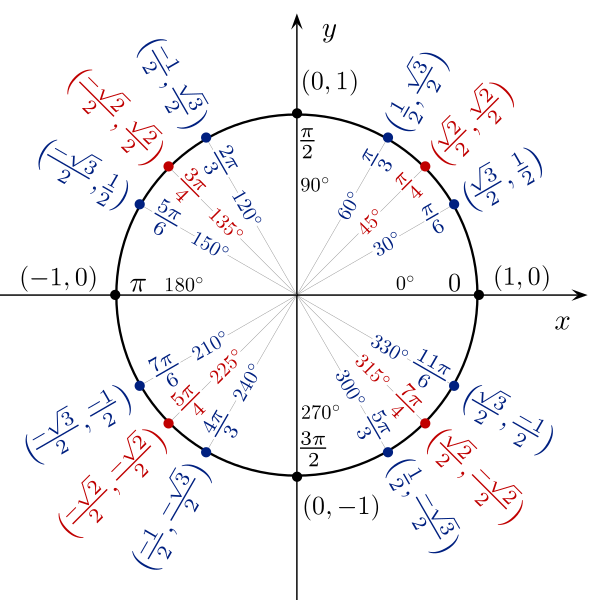
\includegraphics[width=7cm]{angles}

\textbf{Matrix Determinante}

\[
    \begin{vmatrix}
        a & b\\
        c & d
    \end{vmatrix} = ad-bc
\]

\textbf{Matrix Invertierbarkeit}: Eine quadratische Matrix ist genau dann invertierbar, falls die Determinante $\neq 0$.

\textbf{Matrix positiv definit}: Alle Eigenwerte $\lambda_1, ..., \lambda_n > 0$, \textbf{negativ definit:} Alle Eigenwerte $\lambda_1, ..., \lambda_n < 0$, \textbf{indefinit:} Eigenwerte sind positiv und negativ.\\

\textbf{Skalarprodukt} \[ x \cdot y = \sum_{i=1}^n x_i y_i \]

\textbf{TODO! Partielle Integration}

\newpage
\section{Differentialgleichungen}

\begin{Definition}{Differentialgleichung}{}
    Eine \textbf{Differentialgleichung} ist eine Gleichung, in welcher eine unbekannte Funktion $y(x)$ einer oder mehreren Variablen und ihre Ableitung vorkommnt. Im Falle, dass $y$ eine auf dem Intervall $I \subset \R$ definierte Funktion ist \[y: I \subset \R \to \R,\] spricht man von einer \textbf{gewöhnlichen Differentialgleichung}.
\end{Definition}

\begin{Definition}{Ordnung, linear, homogen}{}
    Die \textbf{Ordnung} einer Gleichung ist die höchste vorkommende Ableitung. Bsp: $y''$ $\implies$ 2.\\
    
    Eine Differentialgleichung heisst \textbf{linear}, falls jeder Term $y$, $y'$, $y''$ usw. nur linear vorkommt. Wichtig: Falls $y_1(x)$ und $y_2(x)$ Lösungen der selben Differentialgleichung sind, dass ist auch die Linearkombination $ay_1(x) + by_2(x)$.\\
    
    Eine Differentialgleichung heisst \textbf{homogen}, falls keine Terme vorkommen, die rein von den Funktionsvariablen abhängen (also kein $y$, $y''$, ... enthalten). Sonst heisst die Gleichung \textbf{inhomogen}.
\end{Definition}

\begin{Definition}{Anfangswertproblem}{}
    Ein \textbf{Anfangswertproblem} $n$-ter Ordnung ist eine gewöhnliche Differentialgleichung $n$-ter Ordnung zusammen mit $n$ Anfangsbedingungen.
\end{Definition}

\begin{Satz}{Grundprinzip für lineare, inhomogene Differenzialgleichungen}{}
    Die allgemeine Lösung einer linearen, inhomogenen Differentialgleichung hat die Form
    \[
        \underbrace{y(x)}_{\text{Gesamtlösung}}
        = \underbrace{y_{hom}(x)}_{\text{allg. homogene Lösung}}
        + \underbrace{y_p(x)}_{\text{partikuläre Lösung}}
    \]
    
\end{Satz}

\begin{Rezept}{Separation der Variablen}{}
	Diese Methode eignet sich für \textbf{Differentialgleichungen erster Ordnung} und ist die einfachste Methode.
	
	Für eine Differentialgleichung der Form
	\begin{equation*}
	y' =\frac{dy}{dx}= h(x)\cdot g(y), \qquad \text{mit } g(y)\neq 0
	\end{equation*}
	gehen wir folgendermassen vor:
	\begin{enumerate}
		\item Wir nehmen alle Teile mit $x$ und alle mit $y$ auf verschiedene Seiten.
		\begin{equation*}
		\frac{1}{g(y)} dy=h(x)dx
		\end{equation*}
		\item Nun integrieren wir direkt
		\begin{equation*}
		\int \frac{1}{g(y)}dy = \int h(x) dx
		\end{equation*}
		\item Durch die Unbestimmtheit der Integrale führen wir eine Konstante $C$ ein. Durch Anfangsbedingungen $y(x_0)=y_0$ (in einem Anfangswertproblem) kann diese bestimmt werden.
	\end{enumerate}
\end{Rezept}

\begin{Rezept}{Variation der Konstanten (1. Ordnung)}{}
	Diese Methode eignet sich für \textbf{inhomogene Differentialgleichungen erster Ordnung}, der Form
	
	\begin{equation*}
	y' = h(x) y + b(x).
	\end{equation*}
	
	Wir benutzen den Grundsatz für inhomogene Differentialgleichungen. D.h. wir suchen die allgemeine homogene Lösung und eine partikuläre Lösung und addieren diese für die gesamte Lösung. Eine partikuläre Lösung kann manchmal erraten werden, ansonsten nutzen wir folgendes Rezept:
	
	\begin{enumerate}
		\item Die homogene Lösung $y_{hom}(x)$ suchen wir mit der Methode \textit{Separation der Variablen}.
		\item Die Integrationskonstante aus Schritt I fassen wir als eine von $x$ abhängige Funktion auf
		\begin{equation*}
		C \rightarrow C(x)
		\end{equation*}
		\item Die entstandene Funktion $y_p(x)$ (homogene Lösung mit $C(x)$ anstelle von $C$) setzen wir als Ansatz in die Differentialgleichung ein und lösen nach $C(x)$ auf. Dies gibt uns die partikuläre Lösung.
		\item  Wir nutzen den Grundsatz für die gesamte Lösung
		\begin{equation*}
		y(x) = y_h(x) + y_p(x).
		\end{equation*}.
	\end{enumerate}
\end{Rezept}

\begin{Rezept}{Euler-Ansatz}{}
	Für lineare, homogene Differentialgleichung $n-ter$ Ordnung mit konstanten Koeffizienten, können wir den \textbf{Euler-Ansatz} verwenden. Wir haben eine Gleichung der Form
	\begin{equation*}
	a_n y^{(n)} + a_{n-1} y^{(n-1)} + \dots + a_0 y = 0,
	\end{equation*}
	wobei $a_0,\dots, a_n \in \R$ und $a_n\neq 0$ sind.
	
	Wir wenden folgendes Rezept an:
	\begin{enumerate}
		\item Setze den \textbf{Euler-Ansatz} $y(x) = e^{\lambda x}$, $\lambda \in\mathbb{C}$ in die Differentialgleichung ein und berechne das \textbf{charakteristische Polynom}.
		\item Finde die Nullstellen $\lambda_k$ mit Vielfachheiten $m_k$ des charakteristischen Polynoms und konstruiere daraus die linear unabhängigen Lösungen gemäss
		\begin{equation*}
		e^{\lambda x}, x \cdot e^{\lambda x}, x^2 \cdot e^{\lambda x}, \dots, x^{m-1} \cdot e^{\lambda x}.
		\end{equation*}
		\item Diese Lösungen bilden ein \textbf{Fundamentalsystem} der Differentialgleichung.
		\item Die allgemeinste Lösung ist eine Linearkombination aller Lösungen im Fundamentalsystem. Die Koeffizienten sind durch die Anfangsbedingungen zu bestimmen.
	\end{enumerate}
\end{Rezept}

\begin{Rezept}{Euler-Ansatz mit vielfachen/komplexen Nullstellen}{}
    \begin{tabular}{c|c}
         \textbf{Lösung für $\lambda$} & \textbf{Linearkombinationen um $y(x)$ zu finden}\\
         $\alpha$ & ${\color{green}c_1} \cdot e^{\alpha x}$\\
         $\alpha_1 = \alpha_2 = \ldots = \alpha_k$ & ${\color{green}c_1} \cdot e^{\alpha x} + {\color{blue} x} \cdot e^{\alpha x} + \ldots + {\color{green}c_k} \cdot {\color{blue} x^{k-1}} \cdot e^{\alpha x}$\\
         $\alpha + \beta i, \; \beta>0$ & ${\color{green}c_1} \cdot e^{\alpha x} \cdot \sin(\beta x)$\\
         $\alpha + \beta i, \; \beta<0$ & ${\color{green}c_1} \cdot e^{\alpha x} \cdot \cos(\beta x)$\\
         $\alpha_1 + \beta_1 i = \ldots = \alpha_k + \beta_k i \;\; \beta>0$ & ${\color{green}c_1} \cdot e^{\alpha x} \cdot \sin(\beta x) + \ldots + {\color{green}c_k} \cdot {\color{blue} x^{k-1}} \cdot e^{\alpha x} \cdot \sin(\beta x)$\\
         $\alpha_1 + \beta_1 i = \ldots = \alpha_k + \beta_k i \;\; \beta<0$ & ${\color{green}c_1} \cdot e^{\alpha x} \cdot \cos(\beta x) + \ldots + {\color{green}c_k} \cdot {\color{blue} x^{k-1}} \cdot e^{\alpha x} \cdot \cos(\beta x)$\\
    \end{tabular}
\end{Rezept}

\begin{Diverses}{}{}
	Manchmal sind die Terme in $y(x) = Ae^{ix} + Be^{-ix}$ nicht die geeignetste Form und man möchte lieber reelle Funktionen. Dann nutzt man die Formel 
	\[
		\sin x = \frac{e^{ix} - e^{-ix}}{2i} \quad
    	\cos x = \frac{e^{ix} + e^{-ix}}{2}
    \]
	Damit lassen sich zwei neue Integrationskonstanten definieren: \[\widetilde{A} \sin x + \widetilde{B} \cos x\]
	
	\textbf{Rezept:} Für kompliziertere Ausdrücke funktioniert:
	\[
	    y(x) = Ae^{2ix} + Be^{-2ix} = \widetilde{A} \sin (2x) + \widetilde{B} \cos (2x)
	\]
\end{Diverses}

\begin{Rezept}{Variation der Konstanten (2. Ordnung)}{}
	Wir suchen die Lösung für eine Differentialgleichung der Form
	\begin{equation*}
	y'' + a_1 y' + a_0 y = g(x)
	\end{equation*}
	\begin{enumerate}
		\item Die homogene Lösung $y_h(x)$ finden wir mittels \textbf{Euler-Ansatz}.
		\item Wir suchen nun eine Lösung der Form $y_p(x) = C_1(x) y_1(x) + C_2(x) y_2(x)$, wobei $y_1(x)$ und $y_2(x)$ aus dem Euler-Ansatz stammen und das System
		\begin{equation*}
		\begin{cases} C_1'(x)y_1(x) + C_2'(x)y_2(x)=0\\C_1'(x)y_1'(x) + C_2'(x)y_2'(x)=g(x)\end{cases}
		\end{equation*}
		d.h.
		\begin{equation*}
		\underbrace{\begin{pmatrix}
			y_1(x) &y_2(x)\\y_1'(x) &y_2'(x)
			\end{pmatrix}}_{=:A} \cdot \vekk{C_1'(x)}{C_2'(x)} = \vekk{0}{g(x)}
		\end{equation*}
		erfüllt sein muss. Wir prüfen also, ob die Determinante
		\begin{equation*}
		\det A = y_1(x)y_2'(x)-y_2(x)y_1'(x)
		\end{equation*}
		nicht verschwindet, denn aus LinAlg wissen wir, dass genau dann eine eindeutige Lösung existiert.
		\item  Wir finden nun $C_1$ und $C_2$ und somit $y_p(x)$ entweder durch
		\begin{enumerate}[(a)]
			\item Inversion der Matrix \begin{equation*}
			\vekk{C_1'(x)}{C_2'(x)} = \frac{1}{y_1(x)y_2'(x)-y_2(x)y_1'(x)} \begin{pmatrix}
			y_2'(x) & -y_2(x)\\-y_1'(x) &y_1(x)
			\end{pmatrix}\cdot\vekk{0}{g(x)}
			\end{equation*}
			und anschliessender Integration $C_1 = \int C_1'(x) dx$, $C_2 = \int C_2'(x) dx$ 
			\item oder mit der direkten Formel
			\begin{equation*}
			y_p(x) = -y_1(x) \int \frac{y_2(x) g(x)}{y_1(x)y_2'(x)-y_2(x)y_1'(x)} dx + y_2(x) \int \frac{y_1(x) g(x)}{y_1(x)y_2'(x)-y_2(x)y_1'(x)}dx.
			\end{equation*}
		\end{enumerate}
		\item Die gesamte Lösung erhalten wir aus $y(x) = y_h(x) + y_p(x)$.
	\end{enumerate}
	
	\textbf{Nützliches:} Bei unchilligen Formeln kann $x\mapsto e^t, x^2\mapsto e^{2t},...$ substituiert werden und anschliessend durch ein Gleichungssystem aufgelöst werden.
\end{Rezept}

\begin{Rezept}{Substitution}{}
	\textbf{Gleichungen der Form} $\boxed{y'=h\left(\frac{y}{x}\right)}$\\
	Substitution
	\begin{equation*}
	z(x)=\frac{y(x)}{x} \qquad \Leftrightarrow \qquad y(x)=x z(x),
	\end{equation*}
	dann wird $y'$ durch
	\begin{equation*}
	y'=z+xz'
	\end{equation*}
	ersetzt.\\
	
	\textbf{Gleichungen der Form} $\boxed{y'=h(ax+by+c)}$\\
	Substitution
	\begin{equation*}
	z(x)=ax+by(x)+c \qquad \Leftrightarrow \qquad y=\frac{z-ax-c}{b},
	\end{equation*}
	dann wird $y'$ durch
	\begin{equation*}
	y'=\frac{z'-a}{b}
	\end{equation*}
	ersetzt.\\
	
	\textbf{Gleichungen der Form} $\boxed{y'=h\left(\frac{ax + by + c}{dx + ey + f}\right)}$\\
	Wir wollen $y(x)$ und $x$ ersetzen. Wir lösen das Gleichungssystem
	\begin{equation*}
	\begin{cases}
	ax+by+c=0\\dx+ey+f=0
	\end{cases}
	\end{equation*}
	und wollen eine eindeutige Lösung $(x_0,y_0)$, d.h. wir fordern
	\begin{equation*}
	\det \begin{pmatrix}a &b \\d &e\end{pmatrix}\neq 0.
	\end{equation*}
	Jetzt setzen wir \begin{equation*}
	z=y-y_0 \qquad \text{und} \qquad t=x-x_0.
	\end{equation*}
	Dann werden $y'$ und $z'$ zu 
	\begin{equation*}
	y'=\frac{dy}{dx} = \frac{d(z+y_0)}{d(t+x_0)} = \frac{dz}{dt} = z'.
	\end{equation*}\\
	\textbf{Gleichungen der Form} $\boxed{y'=\frac{y}{x}h(xy)}$\\
	Substitution 
	\begin{equation*}
	z(x)=xy(x) \qquad \Leftrightarrow \qquad y=\frac{z(x)}{x},
	\end{equation*}
	dann wird $y'$ durch
	\begin{equation*}
	y'=\frac{xz'-z}{x^2}
	\end{equation*}
	ersetzt.\\
\end{Rezept}

\begin{Rezept}{Methode des direkten Ansatzes}{}
	Der Ansatz ist geeignet für lineare, inhomogene DGLs $n$-ter Ordnung mit konstanten Koeffizienten. Also eine DGL der Form
	\begin{equation*}
	a_n y^{(n)} + a_{n-1} y^{(n-1)}+\cdots+a_0y = b(x).
	\end{equation*}
	Die homogene Lösung finden wir mit dem Euler-Ansatz. Für die partikuläre Lösung nutzen wir folgende Idee:
	\begin{center}
		$\boxed{\text{Der Ansatz für } y_p(x) \text{hat dieselbe Form wie der inhomogene Term } b(x).}$
	\end{center}
	\begin{center}
		\begin{tabular}{|c|c|}
			\hline 
			Inhomogener Term $b(x)$ & Ansatz für $y_p(x)$ \\ 
			\hline \hline
			$\sum_{i=0}^m b_i x^i$ &	$\sum_{i=0}^m A_i x^i$  \\ 
			$e^{\alpha x}\sum_{i=0}^m b_i x^i$& $e^{\alpha x} \sum_{i=0}^m A_i x^i$ \\ 
			$\sin(\omega x)\sum_{i=0}^m b_i x^i + \cos(\omega x)\sum_{i=0}^m c_i x^i$ &  	$\sin(\omega x)\sum_{i=0}^m A_i x^i + \cos(\omega x)\sum_{i=0}^m B_i x^i$\\ 
			$\sinh(\omega x)\sum_{i=0}^m b_i x^i + \cosh(\omega x)\sum_{i=0}^m c_i x^i$ &  	$\sinh(\omega x)\sum_{i=0}^m A_i x^i + \cosh(\omega x)\sum_{i=0}^m B_i x^i$ \\ 
			$e^{\alpha x}\sin(\omega x)\sum_{i=0}^m b_i x^i + e^{\alpha x}\cos(\omega x)\sum_{i=0}^m c_i x^i$ &  	$e^{\alpha x}\sin(\omega x)\sum_{i=0}^m A_i x^i + e^{\alpha x}\cos(\omega x)\sum_{i=0}^m B_i x^i$\\ 
			\hline 
		\end{tabular} 
	\end{center}
	\textbf{Bemerkung I:} Verschiedene Ansätze können additiv kombiniert werden. So wählt man für $b(x)=5x + \sin(x)e^{3x}$ als Ansatz
	\begin{equation*}
	y_p(x) = \underbrace{Ax + B}_{\text{Teil I}} + \underbrace{(C+\sin x + D \cos x)e^{3x}}_\text{Teil II}.
	\end{equation*}
	\textbf{Bemerkung II:} Wenn ein Teil der für $y_p(x)$ zu wählende Funktion bereits in der Lösung des homogenen Problems vorhanden ist, wird der Ansatz zusätzlich mit $x$ multipliziert. Wenn z.B. die homogene Lösung die Form $y_h(x) = Ax + B$ hat, wählt man anstelle des Ansatzes $y_p(x) = ax+b \Rightarrow y_p(x) = x\cdot(ax+b)$.
\end{Rezept}

\begin{Rezept}{Inhomogene AWP}{}
    Wie im Beispiel ($y' + y = 2\sin(x)$ mit $y(0)=0$) vorgehen:
	\begin{enumerate}
	    \item { Homogene Lösung finden: $(\lambda+1)(e^{\lambda x}) = 0 \Rightarrow \lambda = -1 \Rightarrow y_h = c_1 \cdot e^{-x}$ }
	    \item { Gemäss Störfunktion den Ansatz für $y_p$ wählen und dessen
            Ableitungen finden:
            \begin{align*}
              y_p & = c\cdot \sin(x) + d\cdot \cos(x)\\
              y_p' & = c\cdot \cos(x) - d\cdot \sin(x) 
            \end{align*}
	        }
	    \item { Dies in die ursprüngliche DGL einsetzen, um die Koeffizienten des Ansatzes und damit die partikuläre Lösung zu finden:
	       \[ c \cdot \cos(x) - d\cdot \sin(x) + c\cdot \sin(x) + d\cdot \cos(x) \stackrel{!}{=} 2\sin(x)\] \[ \Leftrightarrow (c+d) \cos(x) + (c-d) \sin(x) \stackrel{!}{=} 2\sin(x) ~ \Longleftrightarrow ~ c=1,\;d=-1 \]
	    }
	    \item{
	        Anfangswertbedingungen nutzen um $c_k$ aus der homogenen Lösung zu finden
	        \[ y(0) = \underbrace{c_1 \cdot e^{-x}}_{y_h(0)} + \underbrace{\sin(x)-\cos(x)}_{y_p(0)} = c_1\cdot1 + 0 - 1 \stackrel{!}{=} 0 \Leftrightarrow c_1 = 1 \]
	    }
	    \item{
	        \[ y(x) = 1 + sin(x) - cos(x) \] 
	   }
	\end{enumerate}
\end{Rezept}

%\subsection{Ordinary Differential Equations}

%\subsection{Linear Differential Equations}

%\subsubsection{Linear Differential Equations of Order 1}

%\subsubsection{Linear Differential Equations with constant coefficients}

%with multiple roots, without multiple roots\\

%rezept von übung


\newpage
\section{Differentialrechnung in $\R^d$}

\subsection{Allgemein}
\textbf{Beschränkt (bounded)} Falls $||x||$ beschränkt für alle $x \in M$.

\textbf{Geschlossen (closed)} Jede Folge $(x_n)$ mit $x_n \in M$ ist $\lim (x_n) \in M$.

\textbf{Kompakt (compact)} Falls beschränkt und geschlossen.

\begin{Definition}{Grenzwert einer Folge in $\mathbb{R}^n$}{}
Für $k\geq1, x_k=(x_{k,1},\cdots,x_{k,n})$ und $y_0 = (y_{0,1}, \cdots, y_{0,n}) $: 
\begin{align*}    
\boxed{\lim\limits_{k \rightarrow +\infty}{x_k} = y_0} \iff &\forall \epsilon > 0 \, \exists k_0 > 0, \text{if } k \geq k_0, ||x_k - y_0|| < \epsilon\\
&\text{or } \lim\limits_{k \rightarrow +\infty}{||x_k-y_0||} = 0\\
&\text{or For } i=1,\cdots, n; \lim\limits_{k \rightarrow +\infty}{x_{k,i}} = y_{0,i}
\end{align*}

\end{Definition}
\subsection{Stetigkeit}

\begin{Definition}{Stetigkeit (Continuity)}{}
    Normale Definition:
    \[
    \lim_{x\rightarrow x_0} f(x) = f(x_0)
    \]
    Definition Stetigkeit mit Folgen: Für jede Folge $(x_n)$ sodass $x_n \rightarrow x$ für $x\rightarrow \infty $:
    \[
    (f(x_n)) \rightarrow f(x)
    \]
\end{Definition}

Sei $f,g$ stetig: $f+g$, $f\cdot g$, $\frac{f}{g}$, $f \circ g$ stetig.

Falls $f$ stetig, gilt

\[
    \lim_{x \rightarrow a} f(x) = f(\lim_{x\rightarrow a} x)
\]

$f$ diffbar $\Rightarrow$ $f$ stetig $\Rightarrow$ $f$ integrierbar

$f$ nicht integrierbar $\Rightarrow$ $f$ nicht stetig $\Rightarrow$ $f$ nicht diffbar.\\

\begin{Rezept}{Polarkoordinatentrick (Change of Variable, Coordinates)}{}
    Ziel: Zeige oder widerlege Stetigkeit. Seien $x=r\cos \varphi$, $y=r\sin \varphi$. Berechne
    \[
    \lim_{(x, y) \rightarrow (0,0)} f(x, y) = \lim_{r \rightarrow 0} f(x, y)
    \]
    Hängt das Resultat von $\varphi$ ab $\Rightarrow$ der Grenzwert existiert nicht $\Rightarrow$ nicht stetig an dieser Stelle.
\end{Rezept}

\begin{Rezept}{Linientrick}{}
    Ziel: Stetigkeit widerlegen. Suche zwei Linien, die einen unterschiedlichen $\lim$ haben. Zeigt, dass ein $\lim$ nicht existieren kann.
    Sei $f(x, y)=\frac{y}{x+1}$ und $\{(x, y) \in \mathbb{R} \mid x \neq 1\}$ für $(x, y) \rightarrow (-1, 0)$. Linie $\{(x, y) \in \mathbb{R} \mid y=0\cap x \neq 1\}=0$ und $\{(x, y) \in \mathbb{R} \mid y=x+1\}=1$.\\
    
    \textbf{Bemerkung:} Meistens à la: $f(x,y)$ verschwindet auf der Linie $\{x=...\}$, dann müsste $\lim_{(x,y)\rightarrow(0,0)} f(x,y) = 0$, aber für $x=...y...$ sehen wir, dass
    $f(x,y) =$ fancy Expression = $1 \neq 0$. Da $x=...$ auf der Linie liegt, folgt der Widerspruch.
\end{Rezept}

\begin{Rezept}{Stetigkeit prüfen}{}
    Sei $f$ die zu prüfende Funktion. 1) $f$ muss überall definiert sein. 2) $\lim_{x \rightarrow a} f(x)$ existiert. 3) $\lim_{x \rightarrow a} f(x) = f(a)$.
\end{Rezept}

\subsection{Differenzierbarkeit}

\begin{Definition}{Differenzierbarkeit}{}
    Sei $\Omega \subset \R$ offen, $f$ : $\Omega \to \R$, $x_0\in\Omega$. $f$ heisst \textbf{differenzierbar an Stelle $x_0$}, falls der Grenzwert
    \[
    \lim_{x\ to x_0} \frac{f(x) - f(x_0)}{x - x_0} =:
    f'(x_0) =:
    \frac{df}{dx}
    \]
    existiert. Wir nennen $f'(x_0)$ die Ableitung (das \textbf{Differential}) von $f$ an der Stelle $x_0$. Eine solche Funktion heisst dann \textbf{differenzierbar auf $\Omega$}, wenn sie an jeder Stelle $x_0 \in \Omega$ differenzierbar ist.
\end{Definition}

$f$ diffbar $\Leftrightarrow$ alle Teil-$f$ sind diffbar.

$f,g$ diffbar $\Rightarrow$ $f+g$, $f \cdot g$, $\frac{f}{g}$, $g \circ f$ diffbar

\begin{Satz}{Kettenregel}{}
	Seien $X,Y \subset \R^n$ offen und $f: X \to Y$, $g: Y \to \R^p$ differenzierbar. Dann ist $g \circ f$ differenzierbar und die Ableitung ist \[d(g\circ f)(x_0) = dg(f(x_0))\circ df(x_0)\] und die Jakobi-Matrix ist \[J_{g\circ f}(x_0) = J_g(f(x_0))J_f(x_0)\]
\end{Satz}


\begin{Definition}{Partielle Differenzierbarkeit}{}
	$f$: $\R^n \rightarrow \R^m$, falls:

	\[
    	\lim_{h \rightarrow 0} \frac{f(x_0 + h e_i)-f(x_0)}{h} =: \frac{\partial f}{\partial x_i}(x_0)
	\]

	oder generell für alle Einheitsvektoren $e_i$ zusammengefasst in Richtung $v \in \R^n$

	\[
    	\lim_{h \rightarrow 0} \frac{f(x_0 + h v)-f(x_0)}{h} =: D_v f(x_0)
	\]

	Dieser $\lim$ existiert $\Leftrightarrow$ in Richtung $e_i$ an Stelle $x_0$ partiell differenzierbar.
\end{Definition}

\begin{Definition}{Totale Differenzierbarkeit}{}
	Sei $f: \Omega \subset \R^m \to \R^n$. $f$ heisst differenzierbar an der Stelle $x_0 \in \Omega$, falls eine lineare Abbildung $A: \R^n \to \R^m$ existiert (also eine $m \times n$ Matrix), sodass \[\lim_{x \to x_0} \frac{|f(x) - f(x_0) - A(x - x_0)|}{|x - x_0|} = 0\] Dann heisst $df(x_0) := A$ das Differenzial von $f$ in Punkt $x_0$. \\
	Diese Matrix $A = Df(x_0)$ ist gegeben durch
	\[
		\text{D}f(x_0) =
        \begin{pmatrix}
            \frac{\partial f_1}{\partial x_1}(x_0)&\hdots&\frac{\partial f_1}{\partial x_n}(x_0)\\
            \vdots&\ddots&\vdots\\
            \frac{\partial f_m}{\partial x_1}(x_0)&\hdots&\frac{\partial f_n}{\partial x_m}(x_0)
        \end{pmatrix}
    \]
\end{Definition}

Prop. 3.4.7!


%TODO study stetigkeit

\subsection{Stetigkeit vs Differenzierbarkeit}

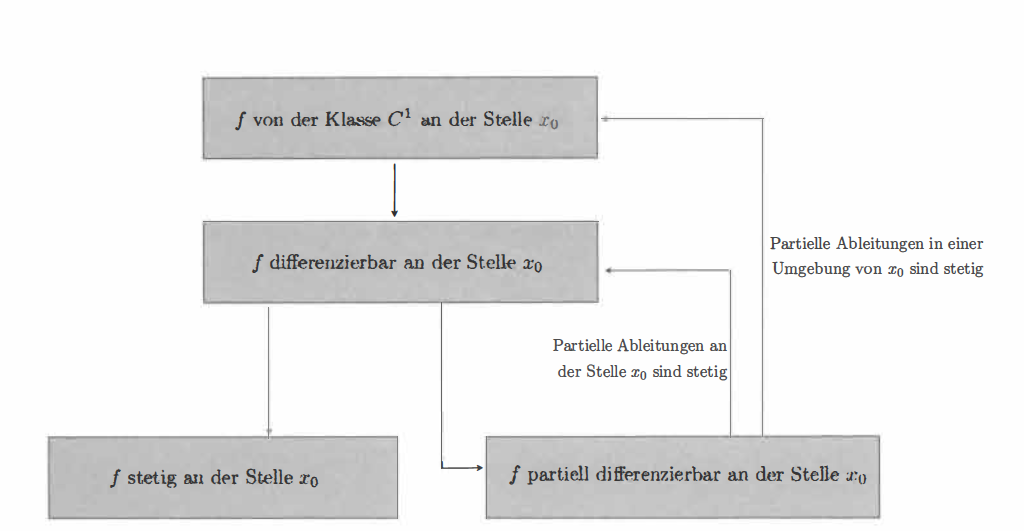
\includegraphics[width=8cm]{1}

\textbf{Prüfen, ob $f$ diffbar and $x_0$}:

$f$ stetig an $x_0$? Nein $\Rightarrow$ $f$ nicht diffbar.\\
$\Downarrow$ Ja\\
Ist $f$ in $x_0$ partiell diffbar, existiert $\frac{\partial f}{\partial x_i}(x_0)$? Nein $\Rightarrow$ $f$ nicht diffbar.\\
$\Downarrow$ Ja\\
Ist $\frac{\partial f}{\partial x_i}(x_0)$ stetig? Ja $\Rightarrow$ $f$ ist diffbar!\\
$\Downarrow$ Nein\\
Existiert eine lineare Abbildung $A$: $\mathbb{R}^n \rightarrow \mathbb{R}^m$ sodass $A=\nabla f(x_0)$, also existert:
\[
    \lim_{x\rightarrow x_0} \frac{|f(x)-f(x_0)-\nabla f(x_0) - (x-x_0)|}{||x-x_0||}
\]?
Ja $\Rightarrow$ $f$ ist diffbar!\\
Nein $\Rightarrow$ $f$ ist nicht diffbar.

\subsection{Partielle Ableitung (Partial Derivative)}

$f$: $\R^n \rightarrow \R$ an Stelle $a$ nach $x_i$

\[
    \lim_{h \rightarrow 0} \frac{f(a_1, ..., a_i + h, ..., a_n) - f(a_1, ..., a_i, ..., a_n)}{h} =: \frac{\partial f}{\partial x_i}(a)
\]

\textbf{Wichtig}: Alle anderen $x_i$ werden als konstante behandelt bei Ableitung.

\subsubsection{Satz von Schwarz (Higher derivatives)}

$f \in C^2$. Gilt nur für zwei und drei verschiedene Variablen. Beliebige Potenzen von $x_i$ und $x_j$ möglich.

\[
    \frac{\partial^2 f}{\partial x_i x_j} = \frac{\partial^2 f}{\partial x_j x_i} \forall i, j \in \{1, ..., n\}
\]


\subsubsection{Gradient}

\[
    \nabla f =
        \begin{pmatrix}
            \frac{\partial f}{\partial x_1}\\
            \vdots\\
            \frac{\partial f}{\partial x_n}
        \end{pmatrix} \quad \text{Nur für } f: X \rightarrow \mathbb{R}
\]

Gradient eines Skalarfeldes: Richtung: Richtung des steilsten Anstiegs; Betrag: Stärke des Anstiegs.\\

\textbf{Regeln} ($n \in \mathbb{N}$, $c$ konstant, $u, v$ Vektoren):
\begin{align*}
    &\text{grad}(c) = 0 &
    &\text{grad}(c \cdot u) = c \cdot \text{grad}(u) \text{  (Linearität)} \\
    &\text{grad}(u + v) = \text{grad}(u) + \text{grad}(u) \text{  (Addition)} &
    &\text{grad}(u \cdot v) = \text{grad}(u) \cdot \text{grad}(u) 
    \text{  (Produktregel)} \\
    &\text{grad}(u^n) = n \cdot u^{n-1} \cdot \text{grad}(u) (n\neq 0) 
\end{align*}
\subsubsection{Richtungsableitung (Directional Derivative)}

$f$ heisst an der Stelle $a$ in Richtung $u$ differenzierbar, falls der Grenzwert 
	\[
		\lim_{h\to0}\frac{f(a + hu) -f(a)}{h} =
		\left.\frac{d}{dh}f(a+hu)\right|_{h = 0}
		=: D_vf(a)
	\]
existiert (oder $g(h) = f(x_0 + hu)$). Ist $||u|| = 1$ (normiert), heisst dieser Grenzwert Richtungsableitung.

\begin{Rezept}{Richtungsableitung $D_uf(a)$ existiert:}{} Falls $t \mapsto f(a + tu)$ differenzierbar ist bei $t=0$, dann existiert $D_uf(a)$.\\

	Die Richtungsableitung existiert für \textbf{jede Richtung}, falls $\left.\frac{d}{dh} f(a + hu) \right|_{h=0}$ NICHT von $\varphi$ abhängt (wenn mal $x=r\cos(\varphi)$, $y=r\sin(\varphi)$ substituiert).
\end{Rezept}

\begin{Rezept}{Richtungsableitung $D_u f(a)$}{}
Falls $f$ in $a$ differenzierbar ist: Für $f$ in Richtung $u$ in Punkt $a$: 1) $u$ normieren: $\tilde{u} = \frac{u}{\|u\|}$ 2) Gradient $\nabla f(x)$ berechnen, dann:

\[
    D_u f(a) = \tilde{u} \underbrace{\cdot}_{\text{SP.}} \nabla f(a)
\]
\end{Rezept}
\begin{Rezept}{Change of variable}{}
$g$ drückt jede Variable $x_i$ von $f$ mit neuen Variablen $(y_1, ..., y_n)$ aus.
\[
U \subset \mathbb{R}^n \text{ offen } \xrightarrow{g}  V \subset \mathbb{R}^n \text{ offen }
\]
Ableitungen:
\[
\frac{\partial h (y)}{\partial y_i} = \frac{\partial f(g(y)))}{\partial x_1} \cdot \frac{\partial g_1(y)}{\partial y_i} \cdots \frac{\partial f(g(y))}{\partial x_n} \cdot \frac{\partial g_n(y)}{\partial y_i}
\]
In der Notation wird $h$ durch $f$ ersetzt und $g_i$ durch $x_i$.
\end{Rezept}
Beispiel Polarkoordinaten:
\[
g(\iota, \theta) = (\iota \cos{\theta}, \iota \sin{\theta}) \quad
J_g(\iota, \theta) = \begin{pmatrix}
\cos{\theta} & -\iota \sin{\theta} \\ \sin{\theta} & \iota \cos{\theta}
\end{pmatrix}
\]
\[
J_h = J_f \cdot J_g \Rightarrow \partial_\iota h = \dots, \partial_\theta h = \dots \rightarrow \text{Nach $\partial_x f$ und $\partial_y f$ auflösen}
\]

\begin{Diverses}{Koordinatentransformationen}{}
    \textbf{Polarkoordinaten:}
    $\partial_x f = \cos{\theta} \partial_\iota f - \frac{1}{\iota}\sin{\theta}\partial_\theta f \quad
    \partial_x f = \cos{\theta} \partial_\iota f - \frac{1}{\iota}\sin{\theta}\partial_\theta f $\\
    \textbf{Zylinderkoordinaten:} \dots
\end{Diverses}

\begin{Definition}{Hessematrix}{}
\[
    \mathbf{Hess}(f) =
        \begin{pmatrix}
            \frac{\partial^2 f}{\partial x_1^2}&\hdots&\frac{\partial^2 f}{\partial x_1 x_n}\\
            \vdots&\ddots&\vdots\\
            \frac{\partial^2 f}{\partial x_n x_1}&\hdots&\frac{\partial^2 f}{\partial x_n^2}
        \end{pmatrix}
\]
\end{Definition}

\begin{Definition}{Jakobimatrix}{}
\[
    f(x, y) =
        \begin{pmatrix}
            f_1(x, y)\\
            \vdots\\
            f_n(x, y)
        \end{pmatrix} \quad
    \mathbf{J_f}(x, y) =
        \begin{pmatrix}
                \frac{\partial f_1}{\partial x} & \frac{\partial f_1}{\partial y}\\
                \vdots&\vdots\\
            \frac{\partial f_n}{\partial x} & \frac{\partial f_n}{\partial y}
        \end{pmatrix}
\]
Für die Kettenregel von Jakobimatrizen siehe ''generelle Kettenregel''.
\end{Definition}

\begin{Definition}{Laplace Operator}{}
\[
\Delta f = \nabla(\nabla f)) = \sum_{k=1}^{n} \frac{\partial^2 f}{\partial x_k^2} = \text{trace}(\textbf{Hess}(f))
\]
\end{Definition}

\subsection{Taylorpolynome}

\[
    f(x) = f(a) + f'(a)(x-a) + \frac{1}{2} f''(a)(x-a)^2 + \frac{1}{3!} f^{(3)}(a)(x-a)^3 + ...
\]

\textbf{In $\R^2$}: $\Delta x = (x - x_0)$, ~ $\Delta y = (y - y_0)$
\begin{align*}
    \; & f(x, y) =f(x_0, y_0)\\ &+ \frac{\partial f}{\partial x}(x_0,y_0) \Delta x + \frac{\partial f}{\partial y}(x_0,y_0) \Delta y\\
    &+ \frac{1}{2} \left(\frac{\partial^2 f}{\partial x^2}(x_0,y_0) (\Delta x)^2 + 2\frac{\partial^2 f}{\partial x \partial y}(x_0,y_0) \Delta x \Delta y + \frac{\partial^2 f}{\partial y^2}(x_0,y_0) (\Delta y)^2\right)\\
    &+ \frac{1}{3!} \left(\frac{\partial^3 f}{\partial x^3}(x_0,y_0) (\Delta x)^3 + 3\frac{\partial^3 f}{\partial x^2 \partial y}(x_0,y_0) (\Delta x)^2 \Delta y\right.\\
    &\quad\quad\quad\;+ \left.3\frac{\partial^3 f}{\partial x \partial y^2}(x_0,y_0) \Delta x (\Delta y)^2 + \frac{\partial^3 f}{\partial y^3}(x_0,y_0) (\Delta y)^3\right)\\
    & + ...
\end{align*}

\textbf{In $\R^n$}: $\Delta x_i = x_i - x_i^0$
\[
	Tf(x;x_0) = \left.\sum_{n=0}^\infty \frac{1}{n!}\left(\Delta x_1 \frac{\partial}{\partial x_1} + ... + \Delta x_n \frac{\partial}{\partial x_n} \right)^n 
		f(x_1, ..., x_n)\right|_{(x_1^0,...,x_n^0)}
\]

\textbf{In $\R^n$ bis Grad 2}:
\[
    T_2f(x) = f(x_0) + \nabla f(x_0)	 (x-x_0) + \frac{1}{2} (x-x_0)^\top \text{Hess}_f(x_0) (x-x_0) 
\]

\begin{Diverses}{Taylorentwicklungen}{}
    \begin{align*}
    e^z &= \sum_{k=0}^{\infty} \frac{z^k}{k!} = 1 + z + \frac{z^2}{2}+ \frac{z^3}{3!}+ \frac{z^4}{4!} + \cdots & 
    \frac{1}{1 \pm x} &= 1 \mp x + x^2 \mp x^3 + x^4 \mp \cdots\\
    \frac{1}{(1 \pm x)^2} &= 1 \mp 2x + 3x^2 \mp 4x^3 + 5x^4 \mp \cdots &
    \sqrt{1 \pm x} &= 1 \pm \frac{x}{2} - \frac{\scriptstyle{1\cdot 1}}{\scriptstyle{2 \cdot 4}}x^2 \pm \frac{\scriptstyle{1\cdot 1 \cdot 3}}{\scriptstyle{2 \cdot 4 \cdot 6}}x^3 - \frac{\scriptstyle{1 \cdot 1 \cdot 3 \cdot 5}}{\scriptstyle{2 \cdot 4 \cdot 6 \cdot 8}}x^4 \pm \scriptstyle\cdots \\
    \sin(\phi) &= \sum_{k=0}^{\infty} (-1)^k \frac{\phi^{2k}}{(2k)!} = \phi - \frac{\phi^3}{3!} + \frac{\phi^5}{5!} + \cdots &
    \sinh(z) &= \sum_{k=0}^{\infty} \frac{z^{2k+1}}{(2k+1)!} = z + \frac{z^3}{3!} + \frac{z^5}{5!} + \cdots\\
    \cos(\phi) &= \sum_{k=0}^{\infty} (-1)^k \frac{\phi^{2k+1}}{(2k+1)!} = 1 - \frac{\phi^2}{2!} + \frac{\phi^4}{4!} + \cdots &
    \cosh(z) &= \sum_{k=0}^{\infty} \frac{z^{2k}}{(2k)!} = 1 + \frac{z^2}{2!} + \frac{z^4}{4!} + \cdots\\
    \tan(\phi) &= \text{...complicated...} = 1 + \frac{\phi^3}{3} + \frac{2\phi^5}{15} + \cdots&
    \tanh(z) &= \text{...complicated...} = 1 \pmb{-} \frac{z^3}{3} \pmb{+} \frac{2z^5}{15} \pmb{-} \cdots\\
    \ln(1+z) &= \sum_{k=1}^{\infty} \frac{(-1)^{k+1}}{k}z^k = z - \frac{z^2}{2} + \frac{z^3}{3} + \scriptstyle\cdots &
    (1+z)^\alpha& = \sum_{k=0}^{\infty}  \binom{\alpha}{k} z^k = 1 + \alpha z + \frac{\alpha(\alpha - 1)}{2!} z ^ 2 + \scriptstyle\cdots
    \end{align*}
\end{Diverses}

\begin{Rezept}{Tangentialebene (Variante I)}{}
    Tangentialebene der Fläche $f(x, y)$ finden in Punkt $(x_0, y_0)$.
    
    \textbf{Lösungsschritt I:}
    Erstelle $F(x, y) = (x, y, f(x, y))^\top$ und berechne die
    Basisvektoren für die Tangentialebene
    \[
        dF(x_0, y_0) =
            \begin{pmatrix}
                \frac{\partial F_1}{\partial x}(x_0, y_0)&\frac{\partial F_1}{\partial y}(x_0, y_0)\\
                \frac{\partial F_2}{\partial x}(x_0, y_0)&\frac{\partial F_2}{\partial y}(x_0, y_0)\\
                \frac{\partial F_3}{\partial x}(x_0, y_0)&\frac{\partial F_3}{\partial y}(x_0, y_0)
            \end{pmatrix} = 
            \begin{pmatrix}
                u_1&v_1\\
                u_2&v_2\\
                u_3&v_3
            \end{pmatrix}
    \]
    ($x_0$ und $y_0$ einsetzen).\\
    \textbf{Lösungsschritt II:}
    Berechne Normalvektor:
    \[
        n =
        u \times v =
        \begin{pmatrix}
            u_1\\
            u_2\\
            u_3
        \end{pmatrix}
        \times
        \begin{pmatrix}
            v_1\\
            v_2\\
            v_3
        \end{pmatrix} = 
        \begin{pmatrix}
            a\\
            b\\
            c
        \end{pmatrix}
    \]
    Berechne $d$ mit $p=(x_0,y_0,f(x_0,y_0))$:
    \[
        d=p \cdot n
    \]
    \textbf{Lösungsschritt III:} Konstruiere Gleichung, sodass:
    \[
        ax + by + cz = d
    \]
\end{Rezept}

\begin{Rezept}{Tangentialebene (Variante II)}{}
\textbf{Idee}: Annäherung von $f$ im Punkt $(x_0, y_0)$ durch Taylorpolynom I. Grades
\[ z = f(x_0, y_0) + \frac{\partial f}{\partial x}(x_0, y_0)\cdot(x-x_0) + \frac{\partial f}{\partial y}(x_0, y_0)\cdot(y-y_0) \]
kann direkt umgeformt werden in die Normalform der Ebenengleichung.
Allgemein für diffbare $f: X \rightarrow \mathbb{R}$ auf $x_0 \in \mathbb{R}^n$:
\begin{equation*}
    z = f(x_0) + J_f(x_0) \underbrace{\cdot}_{\small{\text{Matrixprod.}}} (x-x_0)
\end{equation*}
\end{Rezept}

\subsection{Extremstellen (Kritische Punkte)}

\begin{Definition}[label=R1]{Kritische und reguläre Punkte}{}
	\textbf{Fall $f: \R^n \to \R$}: Sei 	$f: \Omega \subset \R^n \to \R$ differenzierbar. Ein Punkt $p_0 \in \Omega$ heisst \textbf{kritischer Punkt von $f$}, falls $df(p_0)=0$. Ist der Punkt nicht kritisch, heisst er \textbf{regulär}.\\
	
	\textbf{Fall $f: \R^n \to \R^m$}: Sei $f: \Omega \subset \R^n \to \R^m$ differenzierbar. Wir wissen, dass $df(x_0)$ eine lineare Abbildung ist.
	Diese lässt sich mit einer $m\times n$-Matrix darstellen. Der \textbf{Rang} der Matrix beschreibt die Dimension des Bildes.
	Für eine $m \times n$ Matrix $A$ gilt \[\text{Rang}(A) \leq \min(m, n)\] Ein Punkt $p_0 \in \Omega$ heisst \textbf{regulär},
	wenn die Matrix $df(x_0)$ einen maximalen Rang besitzt. Sonst heisst $p_0$ kritisch.
	Ein kritischer Punkt heisst \textbf{degeneriert}, wenn an dieser Stelle für die Hesse-Matrix gilt:
	\[\det(H_f(p_0)) \neq 0\]
	Ansonsten heisst der Punkt \textbf{nicht-degeneriert}.
\end{Definition}

\begin{Satz}{Extremwerte in einer Variable}{}
	Sei $f: \Omega \subset \R \to \R$, $f \in C^2$ und $x_0 \in \Omega$ ein kritischer Punkt (d. h. $f'(x_0) = 0$), dann gilt
	\begin{itemize}
		\item $x_0$ ist ein Minimum, falls $f''(x_0) > 0$,
		\item $x_0$ ist ein Maximum, falls $f''(x_0) < 0$,
		\item $x_0$ ist ein Sattelpunkt, falls $f''(x_0) = 0$
	\end{itemize}
\end{Satz}

\begin{Satz}{Extremwerte in mehreren Variablen (Corollary 3.8.7)}{}
Sei $X\subset \R^n$ offen und $f: X \rightarrow \R \in C^2$. ~~
Sei $x_0$ ein nicht-degenerierender kritischer Punkt von $f$. Sei $p$ und $q$
die Anzahl der positiven resp. negativen Eigenwerte von $\mathbf{Hess_f}(x_0)$.

\begin{enumerate}
\item Falls $p=n$, bzw. $q=0$ ($\text{Hess}_f(x_0)$ ist \textbf{positiv definit}), besitzt $f$ ein lokales \textbf{Minimum} an $x_0$
\item Falls $q=n$, bzw. $p=0$ ($\text{Hess}_f(x_0)$ ist \textbf{negativ definit}), besitzt $f$ ein lokales \textbf{Maximum} an $x_0$
\item Ansonsten, bzw. $pq\neq 0$, besitzt $f$ kein Extremum an $x_0$. Man sagt deshalb, $f$ besitzt einen \textbf{Sattelpunkt} an $x_0$.
\end{enumerate}
\end{Satz}

\begin{Rezept}{Eigenwerte finden}{}
	Charakteristisches Polynom mittels $\det (A-\lambda I)$ berechnen. Nullstellen des Polynoms sind die Eigenwerte.
\end{Rezept}

\begin{Satz}{Definitheit für symmetrische Hesse-Matrizen (Remark 3.8.8)}{}
\begin{center}Für eine \textbf{symmetrische} Matrix gilt\end{center}
\begin{multicols}{2}
\[ A = \begin{pmatrix}
         a & b\\
         b & d
       \end{pmatrix} \]
\begin{align*}
\textbf{positiv definit} & \Longleftrightarrow a > 0, ~~ ad-b^2>0\\
\textbf{negativ definit} & \Longleftrightarrow a < 0, ~~ ad-b^2>0\\
\textbf{indefinit} & \Longleftrightarrow ad-b^2 < 0
\end{align*}


\[ A = \begin{pmatrix}
         a & b & c\\
         b & e & f\\
         c & f & i\\
       \end{pmatrix} \]
\begin{align*}
\textbf{positiv definit} & \Longleftrightarrow a > 0, ~~ ae-b^2>0, ~~ \det \; A > 0\\
\end{align*}


\end{multicols}


\end{Satz}

\begin{Satz}{Eigenwert-Kriterium}{}
	Seien $\lambda_1, ..., \lambda_n$ die Eigenwerte einer reellen, symmetrischen $n \times n$ Matrix $A$. Dann gilt
	\begin{align*}
		A \text{ ist positiv definit} &\iff \text{Alle }\lambda_i > 0,\\
		A \text{ ist positiv semi-definit} &\iff \text{Alle }\lambda_i \geq 0,\\
		A \text{ ist negativ definit} &\iff \text{Alle }\lambda_i < 0,\\
		A \text{ ist negativ semi-definit} &\iff \text{Alle }\lambda_i \leq 0
	\end{align*}
\end{Satz}

\begin{Definition}{Hauptminoren}{}
	Die Hauptminor einer symmetrischen, reellen Matrix $A$ sind die nordwestlichen Unterdeterminanten der Matrix $A$. Sie werden mit $A_i$ bezeichnet, wobei $i$ die Grösse der Teilmatrix $A_i$ ist. 
	
	Sei die Matrix
	\[
		A = \begin{pmatrix}
            a_{11} & a_{12} & \hdots & a_{1n}\\
            a_{21} & a_{22} & \hdots & a_{2n}\\
            \vdots & \vdots & \ddots & \vdots\\
            a_{n1} & a_{n2} & \hdots & a_{nn}
        \end{pmatrix}
	\]
	dann sind die $n$ Hauptminoren $A_1, ..., A_n$ gegeben durch
	\begin{align*}
		A_1 &= \det(a_{11}) = a_{11},\\
		A_2 &= \det\begin{pmatrix}
            a_{11} & a_{12} \\
            a_{21} & a_{22}
            \end{pmatrix},\\
       	A_3 &= \det\begin{pmatrix}
            a_{11} & a_{12} & a_{13} \\
            a_{21} & a_{22}& a_{23}\\
            a_{31} & a_{32}& a_{33}
            \end{pmatrix},\\
            &\vdots\\
        A_n &= \det(A)
    \end{align*}
\end{Definition}

\begin{Satz}{Sylvester-Kriterium}{}
	\textbf{NUR FÜR GROSSE MATRIZEN VERWENDEN.}
	Sind $A_1, ..., A_n$ die Hauptminoren der reellen, symmetrischen $n \times n$ Matrix A, dann gilt:
	\begin{align*}
		A \text{ ist positiv definit} &\iff \text{Alle }A_i > 0,\\
		A \text{ ist negativ definit} &\iff \text{Wechselndes Vorzeichen: }A_1 < 0, A_2 > 0, A_3 < 0,...\\
		A \text{ ist indefinit} &\iff \text{Weder alle }A_i \leq 0 \text{ noch }A_i \geq 0 
	\end{align*}
\end{Satz}

\begin{Rezept}[label=Skalar1]{Kritische Punkte finden in Skalarfeld (im Inneren, nicht abgegrenzt)}{}
	\textbf{Lösungsschritt I:} Gradient berechnen; Gradient $=0$ setzen $\implies$ kritische Punkte.
	
	\textbf{Lösungsschritt II:} Hessematrix berechnen; für jeden kritischen Punkt: Falls die Hessematrix positiv definit ist $\implies$ lokales Minimum; falls Hessematrix negativ definit ist $\implies$ lokales Maximum; sonst Sattelpunkt.
\end{Rezept}

\begin{Rezept}[label=Skalar2]{Kritische Punkte finden in Skalarfeld (abgegrenzt)}{}
	\textbf{Lösungsschritt I:} Inneres Skalarfeld nach kritischen Punkten untersuchen nach Rezept \ref{Skalar1}. ($\nabla f \stackrel{!}{=} 0$)
	
	\textbf{Lösungsschritt II:} Alle Begrenzungen des Skalarfeldes einzeln nach kritischen Punkten untersuchen. Beispiel Dreieck: alle Seiten parametrisieren und \textbf{alle Eckpunkte einzeln untersuchen}. Parametrisierungen ableiten und die Extrempunkte der Stücke untersuchen; Eckpunkte notieren.
	$\frac{d}{dt}(f \circ \gamma_1) \stackrel{!}{=} 0$, also $t$, resp. die kritischen Punkte so finden.
	
	\textbf{Lösungsschritt III:} Alle gefundenen Punkte miteinander vergleichen und herausfinden, welches die Extrema sind (jeweils die Funktionswerte der Extrempunkte berechnen).
\end{Rezept}

\begin{Rezept}[label=R1]{Extremwertaufgaben ohne Nebenbedingungen}{}
	Gegeben: $f:\Omega\subset \R^n \to \R$ mit $\Omega$ offen (d.h. ohne Rand) und $f$ von der Klasse $C^2$.\\
	Gesucht: Extremalstellen von $f$ in $\Omega$.\\
	\newline
	\textbf{Lösungsschritt I:}\\
	Finde die kritischen Punkte $\{x_0\} \in \Omega$. D.h. alle Punkte, für die gilt
	\begin{equation*}
	df(x_0)=0
	\end{equation*}
	und $x_0 \in \Omega$.\\
	\textbf{Lösungsschritt II:}\\
	Untersuche die Hesse-Matrix von $f$ in den Punkten $\{x_0\}$ um über die Art der Extremum zu entscheiden.
	\begin{align*}
	\text{H}_f(x_0) \text{ ist positiv definit} \qquad &\Rightarrow \qquad x_0 \text{ ist ein lokales Minimum von} f\\
	\text{H}_f(x_0) \text{ ist negativ definit} \qquad &\Rightarrow \qquad x_0 \text{ ist ein lokales Maximum von} f\\
	\text{H}_f(x_0) \text{ ist indefinit} \qquad &\Rightarrow \qquad x_0 \text{ ist ein Sattelpunkt von} f
	\end{align*}
	Wenn die Hesse-Matrix keine klare Aussage ergibt (degenerierte kritische Punkte), muss man die Funktion in einer Umgebung abschätzen (um ein Max/Min zu zeigen) oder konkrete Gegenbeispiele finden.
\end{Rezept}

\begin{Rezept}[label=R2]{Extremwerteaufgaben mit ``einfachen'' Nebenbedingungen}{}
	Gegeben: $f:\Omega\subset \R^n \to \R$ mit Rand $\partial{\Omega}$ und $f$ von der Klasse $C^2$.\\
	Gesucht: Extremalstellen von $f$ in $\Omega$.\\
	\newline
	\textbf{Lösungsschritt I:}\\
	Wir untersuchen das Innere $\overset{\circ}{\Omega}$ analog zu Rezept \ref{R1}.\\
	\newline
	\textbf{Lösungsschritt II:}\\
	Wir parametrisieren den Rand $\partial \Omega$ durch $\gamma(t)$. Die kritischen Punkte sind dann die Punkte $\gamma(t)$ für die gilt
	\begin{equation*}
	\dv{t}(f\circ \gamma)(t) = 0.
	\end{equation*}
	\newline
	\textbf{Lösungsschritt III:}\\
	Bestimme die Art der kritischen Punkte.
	\begin{itemize}
		\item Variante 1 (nur kleinstes Min/ grösstes Max): \\Werte alle kritischen Punkte auf dem Rand explizit aus. D.h. berechne $f(\gamma(t))$.
		\item Variante 2 (Min/Max/Sattelpunkt):\\
		Die Funktion $f(\gamma(t))$ ist nur von einer Variable abhängig. Bestimme die Art der kritischen Punkte anhand der Kriterien für 1D-Funktionen.
	\end{itemize}
	
	\textbf{Lösungsschritt IV:}\\
	Ist der Rand stückweise parametrisiert durch $\gamma_1,\gamma_2,\dots$, muss die Funktion zusätzlich an allen Anfangs- und Endpunkten der $\gamma_i$  explizit ausgewertet werden.\\
	\newline
	\textit{Bemerkung: Das Wort "'einfach"' bedeutet hier, dass wir eine Parametrisierung für den Rand finden können.}
\end{Rezept}

\subsection{Lagrange Multiplikatoren}
Sei $f(x) \in \R^{n}$ die zu maximierende Funktion, von der wir aber nur Punkte
betrachten wollen, für welche gilt, dass $g(x) = 0$ mit $g(x) \in \R^{l}$
Definition der \textbf{Lagrange-Funktion}:
\[ L = f-\lambda \cdot g = f - \lambda_{1} g_{1} - \ldots - \lambda_{n}g_{n} ~ \text{ mit $\lambda$ in } \R^{l} \]
Dieses $\lambda$ existiert immer, wenn $f, g \in C^{1}$.
Die Kandidaten für Extrema von $f$ unter der Nebenbedingung $g = 0$ sind genau die
kritischen Punkte der Lagrange-Funktion $L$. Mittels der Hesse-Matrix von $L$
kann die Art der Extrema gefunden werden. Jeder Kandidat wird in $f$ eingesetzt
um zu erkennen, wo $f$ mit welchen Werten Extrema annimmt.

\begin{Rezept}{Extremwertaufgaben mit Nebenbedingungen}{}
	Gegeben: $f:\Omega\subset \R^n \to \R$ und $g:\Omega \to \R^l$ der Klasse $C^1$.\\
	Gesucht: ein Extremum der Funktion $f$ unter der Nebenbedingung $g=0$.\\
	\newline
	\textbf{Lösungsschritt I:}\\
	Bilde die Lagrange-Funktion
	\begin{equation*}
	L(x_1,\dots,x_n,\lambda) = f(x_1,\dots,x_n) - \lambda_1 g_1(x_1,\dots,x_n) - \dots - \lambda_l g_l(x_1,\dots,x_n),
	\end{equation*}
	wobei $g_1,\dots,g_l$ die $l$ Komponenten von $g$ sind. Oft ist $l=1$.\\
	\newline
	\textbf{Lösungsschritt II:}\\
	Bestimme die kriischen Punkte von L, d.h. löse
	\begin{align*}
	\pdv{L}{x_1} &= \pdv{f}{x_1}-\lambda_1\pdv{g_1}{x_1} - \dots -\lambda_l\pdv{g_l}{x_1} = 0\\
	\vdots\\
	\pdv{L}{x_n} &= \pdv{f}{x_n}-\lambda_1\pdv{g_1}{x_n} - \dots -\lambda_l\pdv{g_l}{x_n} = 0.
	\end{align*}
	
	Löse dieses Gleichungssystem mit den zusätzlichen Gleichungen von $g=0$.\\
	\newline
	\textbf{Lösungsschritt III:}\\
	Die Lösungen $(x_1,\dots,x_n)$ sind die Kandidaten für Extremalstellen von $f$. Untersuche die Hesse-Matrix von L um den Typ zu bestimmen.
	\begin{align*}
	\text{Hess}(L)(x_0,\lambda)\text{ ist positiv definit} &\rightarrow 
	x_0 \text{ ist ein lokales Minimum von } f \text{ auf } g^{-1}(0),\\
	\text{Hess}(L)(x_0,\lambda)\text{ ist negativ definit} &\rightarrow x_0 \text{ ist ein lokales Maximum von } f \text{ auf } g^{-1}(0),\\
	\text{Hess}(L)(x_0,\lambda)\text{ ist indefinit} &\rightarrow x_0 \text{ ist ein Sattelpunkt von } f \text{ auf } g^{-1}(0).
	\end{align*}
	
	Ist man nur an den \textbf{globalen Extremwerten} interessiert, spart man sich diesen Schritt und wertet stattdessen die Funktion $f$ an den Kandidaten aus.\\
	\newline
	\textbf{Lösungsschritt IV:}\\
	Ist man auch an Extremalstellen im Innern $\overset{\circ}{\Omega}$ interessiert, sucht man diese mit dem bereits bekannten Rezept.
\end{Rezept}

TODO: falls no platz: beispiele für extremwertaufgaben mit nebenbedingungen breckman (?)
%%TODO umkehrabbilung

\subsection{Satz der Umkehrabbildung}

theorem 3.10.2\\

%\subsection{Satz der Impliziten Funktion}

Ziel: Existenz von lokalen Umkehrungen. ''Implizit'', weil die Form der Gleichung stets ein Gleichungssystem impliziert. Sei das Gleichungssystem der Form:

\[
    f(x, y) = 0
\]

$x = (x_1, ..., x_k)$, $y = (y_1, ..., y_l)$

\[
    df(x, y) = (df_x(x, y) \mid df_y(x, y)) = 
        \begin{pmatrix}
            \frac{\partial f_1}{\partial x_1} & \hdots & \frac{\partial f_1}{\partial x_k}
            & \frac{\partial f_1}{\partial y_1} & \hdots & \frac{\partial f_1}{\partial y_l}\\
            
            \vdots & \ddots & \vdots & \vdots & \ddots & \vdots\\
            
            \frac{\partial f_l}{\partial x_1} & \hdots & \frac{\partial f_l}{\partial x_k}
            & \frac{\partial f_l}{\partial y_1} & \hdots & \frac{\partial f_l}{\partial y_l}\\
        \end{pmatrix}
\]

\begin{Satz}{Implizite Funktionen}{}
	Sei $\Omega \subset \R^n = \R^k \times \R^l$ offen und sei $f: \Omega \to \mathbb{R}^l$ stetig differenzierbar. Ist der Punkt $p_0 = (a, b) \in \Omega$ (mit $a=$ erste $k$ Koordinaten und $b=$ letzte $l$ Koordinaten von $p_0$) regulär mit
	\[
    	f(p_0) = 0 \text{ und } \det(d_y f(p_0)) \neq 0\ (\iff d_y f(p_0) \text{ ist invertierbar})
	\]
	wobei $d_yf(p_0)$ die partiellen Ableitungen der Koordinaten $y_1, ..., y_l$ enthält, so lässt sich das Gleichungssystem $f(x, y) = 0$ nach Koordinaten $y$ auflösen. Das heisst es existiert ein $h: U \to V$ sodass 
	\[
  		\exists h: f(x, h(x)) = 0
	\]
\end{Satz}

\textbf{Rezept: Ableitung der Auflösungsfunktion $h$:} Bsp 2-dimensional (auflösen nach $y$) oder 3-dimensional (auflösen nach $z$)

\[
    dh(x) = -\frac{d_x f(x, h(x))}{d_y f(x, h(x))}
\]


\[
    \nabla h(x, y) =
        \left(
            -\frac{\partial_x f(x, y, h(x, y))}{\partial_z f(x, y, h(x, y))},
            -\frac{\partial_y f(x, y, h(x, y))}{\partial_z f(x, y, h(x, y))}
        \right)
\]

\textbf{Rezept: Typische Aufgabe} 1. $p_0$ bestimmen, sodass $f(x, y)=0$ stimmt. 2. $df(x, y)$ berechnen und $d_y$ kontrollieren, ob $\neq 0$ 3. Satz bewiesen, Ableiten der Auflösungsfunktion.



\newpage
\section{Integration in $\mathbb{R}^d$}

\subsection{Wegintegrale}

Sei $f: [a, b] \rightarrow \mathbb{R}^{n}$ stetig, d.h. für
\[ f(t) = (f_1(t), ~ \ldots, ~ f_n(t)) \]
jedes $f_i$ stetig, dann ist
\[ \int_a^b f(t) dt = \left( \int_a^b f_1(t) dt, ~ \ldots , ~ \int_a^b f_n(t) dt\right) \in \mathbb{R}^n \]

Für eine parametrisierte Kurve in $\mathbb{R}^n$, d.h.
$\gamma : [a, b] \rightarrow \mathbb{R}^n$, s.d.
\begin{enumerate}
\item{ $\gamma$ stetig}
\item{2. $\exists t_0, \ldots, t_k$, ~ s.d. $t_0 = a < t_i < t_k = b$, ~~ s.d. ~
$\gamma ~ | ~ ]t_i, t_{i-1}[ ~ \in C^1$}
\end{enumerate}
nennen wir $\gamma$ einen Pfad zwischen
$\gamma(a)$ und $\gamma(b)$. 

\begin{Satz}{Länge einer Kurve}{}
	Sei $\gamma$ eine reguläre Kurve $t \to \gamma(t)$ sei $|.|$ die euklidische Norm: Die Länge ist
	\[
  		L(\gamma) = \int_a^b |\gamma'| dt
  	\]
\end{Satz}

\begin{Rezept}{Wegintegrale}{}
	Gegeben: Vektorfeld f von der Klasse $C^1$ und eine Kurve $\gamma \in C^1_{pw}$.
	
	Gesucht: Wegintegral $\int_\gamma f \cdot ds$.\\
	
	\textbf{Lösungsschritt I:}
	
	Parametrisiere $\gamma$, d.h. finde eine Abbildung $\gamma(t) : [a, b] \to \R^n$, $t \to \gamma(t)$.
	
	\textbf{Lösungsschritt II:}
	
	Berechne $\gamma'(t) = \frac{d}{dt} \gamma(t)$. Dabei wird jede Komponente des Vektors $\gamma$ einzeln nach t abgeleitet.
	
	\textbf{Lösungsschritt III:}
	
	Das Wegintegral von $f$ entlang $\gamma$ ist definiert als
	\[
		\int_{\gamma} f(s)\cdot d\vec{s} = 
		\int_a^b \underbrace{\underbrace{f(\gamma(t))}_{\in\mathbb{R}^n}  \cdot 
		\underbrace{\gamma'(t)}_{\in\mathbb{R}^n}}_{\text{Skalarprodukt in } \mathbb{R}} dt  ~
		\in \mathbb{R}
	\]
	und ist unabhängig der gewählten Parametrisierung!
\end{Rezept}

\subsection{Potential}

Intuition: Stärke der Änderung der Richtung der Vektoren in einem Vektorfeld.

\begin{Definition}{Potentialfelder und Potentiale}{}
	Ein Vektorfeld $\vec{v} : \Omega \subset \R^n \to \R^n$ heisst \textbf{Potentialfeld}, falls eine stetig differenzierbare Abbildung $\Phi : \Omega \subset \R^n \to \R$ existiert, sodass \[\vec{v} = \nabla \Phi\] gilt. Das skalare Feld $\Phi$ heisst dann \textbf{Potential} von $\vec{v}$. \textbf{Wichtig:} Es gibt sehr viele Vektorfelder, die sich nicht als Gradient eines skalaren Feldes schreiben lassen (also keine Potentialfelder sind)!
\end{Definition}

\subsection{Konservative Vektorfelder (= Potentialfelder)}
Ein Vektorfeld $V: (x, y) \mapsto (f_1(x), f_2(y))$ ist konservativ (= ein Potentialfeld) wenn es überall definiert
und zusammenhängend (für 2D: keine 'Löcher') ist und gilt, dass $rot \;V = 0$. Es gelten die \textbf{Integrabilitätsbedingungen} \\ 
Für $\mathbb{R}^2$:
\[ \frac{\partial f_1}{\partial x_2} = \frac{\partial f_2}{\partial x_1} \]
Für $\mathbb{R}^3$:
\[ \frac{\partial f_1}{\partial x_2} =  \frac{\partial f_2}{\partial x_1}, 
~~  \frac{\partial f_1}{\partial x_3} = \frac{\partial f_3}{\partial x_1},
~~ \frac{\partial f_2}{\partial x_3} =  \frac{\partial f_3}{\partial x_2}
\]
Für $\mathbb{R}^n$:
\[
	\frac{\partial f_i}{\partial x_j} =  \frac{\partial f_j}{\partial x_i},
	\quad
	\forall i \neq j,
	\quad
	i, j \in \{1,...,n\}
\]

\begin{Satz}{Wegintegrale für Potentialfelder}{}
	Sei $\vec{v} : \Omega \subset \R^n \to \R^n$ ein Potentialfeld mit Potential $\Phi$. Dann gilt für jedes Wegintegrale entlang $\gamma$, dass
	\[
		\int_\gamma \vec{v} \cdot d\vec{s} = 
		\int_a^b \vec{v}(\gamma(t)) \cdot \gamma'(t) dt =
		\Phi(\gamma(b)) - \Phi(\gamma(a))
	\]
	Wir müssen also nur die Potentiale am Anfangs- und Endpunkt der Kurve auswerten! Damit sieht man auch gerade, dass für jede geschlossene Kurve das Wegintegrale eines Potentialfeldes gleich 0 ist. 
\end{Satz}

\begin{Diverses}{Zusammenfassung}{}
	Sei $\vec{v} : \Omega \subset \R^n \to \R^n$ ein stetig differenzierbares Vektorfeld und $\Omega$ einfach zusammenhängend. Folgende Aussagen sind äquivalent:
	\begin{itemize}
		\item $\vec{v}$ ist konservatives Vektorfeld
		\item $\vec{v}$ ist ein Potentialfeld
		\item Für alle geschlossene Kurven gilt $\oint \vec{v} \cdot d\vec{s} = 0$
		\item Das Integral $\int_\gamma \vec{v} \cdot d\vec{s}$ ist unabhängig vom Weg
		\item $\vec{v}$ erfüllt die Integrabilitätsbedingung auf $\Omega$. Für $\R^3$ gilt also $\nabla \times \vec{v} = 0$
	\end{itemize}
\end{Diverses}
\subsection{Sternförmig?}
Zügs zu Star shaped?

\subsection{Integrationsregeln}

\begin{Satz}{Satz von Fubini}{}
    Reduzierung von mehrdimensionalen Integralen auf eine Dimension. Sei $f: [a,b] \times [c, d]$ stetig, dann gilt
    \[ \int_a^b \int_c^d f(x, y) dx ~ dy = \int_c^d \int_a^b f(x, y) dy ~ dx = \int_{[a,b] \times [c, d]} f(x, y) dx ~ dy   \]

    Es sei der Quader $Q = [a_1,a_2] \times [a_2, b_2] \times \dots \times [a_n, b_n]$ mit $f \in C^0(Q)$ gegeben. Dann gilt

    \[
        \int_Q f(x) d\mu(x) = \int_{a_1}^{b_1} dx_1 \int_{a_2}^{b_2} dx_2 \dots \int_{a_n}^{b_n} dx_n f(x_1, x_2,...,x_n)
    \]
\end{Satz}
Die Integrationsreihenfolge darf vertauscht werden.\\

Alternative Schreibweise von $dx ~ dy$: $\mu(x, y)$, $\mu(x+y)$.

\subsection{Normalbereiche in $\mathbb{R}^2$}

Sei $\Omega$ eine beschränkte Teilmenge von $\mathbb{R}^2$. $\Omega$ heisst \textbf{y-Normalbereich}, falls sich $\Omega$ wie folgt darstellen lässt:

\[
    \Omega = \{(x, y) \in \mathbb{R}^2 \mid a \leq x \leq b, f(x) \leq y \leq g(x)\}
\]

wobei $f$, $g$ stetige Funktionen der Variable $x$ sind. Die Rolle von $x$ und $y$ darf vertauscht werden (es existiert also auch ein $x$-Normalbereich).

Sei \[\Omega = \{(x, y) \in \mathbb{R}^2 \mid a \leq x \leq b, f(x) \leq y \leq g(x)\}\] ein Normalbereich mit stetigen Funktionen $f$, $g$ und sei die zu integrierende Funktion $F \in C^0(\Omega)$, dann gilt:

\[
    \int_{\Omega} F d\mu = \int_a^b dx \int_{f(x)}^{g(x)} dy F(x, y)
\]

Das innere Integral wird zuerst ausgewertet.

\begin{Satz}{Substitutionsregeln in einer Dimension}{}
    Sei $f$ eine Riemann-integrierbare Funktion. Für die Berechnung des Integrals
    \[
        \int_a^b f(x) dx
    \]
    führt die Substitution $x \to g(u)$ zu $dx = g'(u)du$ und damit wird das Integral
    \[
        \int_a^b f(x) dx = \int_{g^{-1}(a)}^{g^{-1}(b)} f(g(u)) g'(u) du
    \]
    Das heisst wir haben das Integrationselement $dx$ durch $g'(u)du$ ersetzt und die Grenzen entsprechend angepasst.
\end{Satz}

\begin{Satz}{Substitutionsregeln in $n$ Dimensionen}{}
    Sei $f$ eine Riemann-integrierbare Funktion auf dem Gebit $\Omega \subset \R^n$ und die Koordinatentransformation (Substitution)
    \[
    (x_1,\hdots,x_n) = \Phi(u_1, \hdots,  u_n)
    \]
    oder in Komponenten
    \[
        \vek{x_1}{\vdots}{x_n}
        = \Phi(u)
        = \vek{g_1(u_1,\hdots,u_n}{\vdots}{g_n(u_1,\hdots,u_n)}
    \]
    ist ein $C^1$-Diffeomorphismus. Dann gilt
    \[
        \int_\Omega f(x_1, \hdots, x_n)dx_1\hdots dx_1 = \int_{\widetilde{\Omega}} f(g_1(u), \hdots, g_n(u))|\det d \Phi | du_1\hdots du_n
    \]
    wobei das Gebiet $\widetilde{\Omega} = \Phi^{-1}(\Omega)$ ist. $|det d\Phi|$ ist die \textbf{Funktionaldeterminante}.
\end{Satz}

\begin{Rechenregeln}{Wichtige Koordinatentransformationen und Funktionaldeterminanten}{}
    \begin{itemize}
       \item Polarkoordinaten in $\R^2$ \begin{alignat*}{4}
            x &= r \cos \varphi\quad &&0 \leq r < \infty\quad &&&dxdy = r \cdot drd\varphi\\
            y &= r \sin \varphi\quad &&0 \leq \varphi < 2\pi\quad
        \end{alignat*}
        \item Elliptische Koordinaten $\R^2$ \begin{alignat*}{4}
            x &= r \cdot  a \cos \varphi\quad &&0 \leq r < \infty\quad &&&dxdy = a \cdot b \cdot  r \cdot drd\varphi\\
            y &= r \cdot b \sin \varphi\quad &&0 \leq \varphi < 2\pi\quad
        \end{alignat*}
        \item Zylinderkoordinaten $\R^3$ \begin{alignat*}{4}
            x &= r \cdot  a \cos \varphi\quad &&0 \leq r < \infty\quad &&&dxdydz = r \cdot drd\varphi dz\\
            y &= r \cdot b \sin \varphi\quad &&0 \leq \varphi < 2\pi\quad\\
            z &= z\quad &&\-\infty \leq z < \infty\quad
        \end{alignat*}
        \item Kugelkoordinaten $\R^3$ \begin{alignat*}{4}
            x &= r \cdot \sin \theta \cos \varphi \quad &&0 \leq r < \infty\quad &&&dxdydz = r^2 \sin \theta \cdot drd\theta d\varphi\\
            y &= r \cdot \sin \theta \sin \varphi \quad && 0 \leq \theta < \pi\quad\\
            z &= r \cos \theta \quad &&0 \leq \varphi < 2\pi\quad\quad
        \end{alignat*}
   \end{itemize}
\end{Rechenregeln} 

\newpage
\section{Tricks und Umformungen}
\begin{Rezept}{$f(b)-f(a)$}{}
Falls irgendwo die Differenz einer Funktion auftaucht, kann oft der Fundamentalsatz genutzt werden
\[ f(b)-f(a) = \int_a^b \frac{\partial f}{\partial x} ~ dx \]
\end{Rezept}

\begin{Rezept}{Beweise, dass z(t) konstant ist}{}
\centering
$z(t)$ konstant $\Longleftrightarrow z'(t) = 0$ bzw $\nabla z(t) = \vek{\frac{\partial z_1}{\partial t}}{\vdots}{\frac{\partial z_n}{\partial t}} = \vek{0}{\vdots}{0}$ also $\forall i \in \{1,\hdots,n\} :\frac{\partial z_i}{\partial t} = 0$
\end{Rezept}


\sadfaces


\end{multicols}

\end{document}
